\section{Explaining Type Errors With Traces}
\label{sec:explaining}

A trace, on its own, is likely too detailed to be
a good explanation of the type error. One approach
is to use the witness input to step through the
program with a \emph{debugger} to observe how
the program evolves.
%
This route is problematic for two reasons.
%
First, existing debuggers and interpreters for
typed languages (\eg\ \ocaml) typically require
a type-correct program as input.
%
Second, we wish to have a quicker way to get
to the essence of the error, \eg\ by skipping
over irrelevant sub-computations, and focusing
on the important ones.

Next, we present a novel way to debug executions.
%
First, we develop a notion of a
\emph{reduction graph}~(\S~\ref{sec:reduction-graph}).
%
Second, we extend our semantics with a form of \emph{tracing}
so that they incrementally collect the edges in the graph
(\S~\ref{sec:inter-semant}).
%
Finally, we express a set of common \emph{interactive debugging}
steps as graph traversals (\S~\ref{sec:traversing-graph}), yielding
an novel visual interactive debugger that allows the user
to effectively visualize \emph{how} the program goes (wrong.)

% The trace takes the form of a \emph{reduction graph}, where the nodes
% are terms and the edges represent either the single-step
% $\hookrightarrow$ or a ``sub-term'' relation. For example, evaluating
% the expression @1 + 2 + 3@ would produce the graph in
% Figure~\ref{fig:simple-reduction}.
% %
% \begin{figure}[t]
%   \centering
%   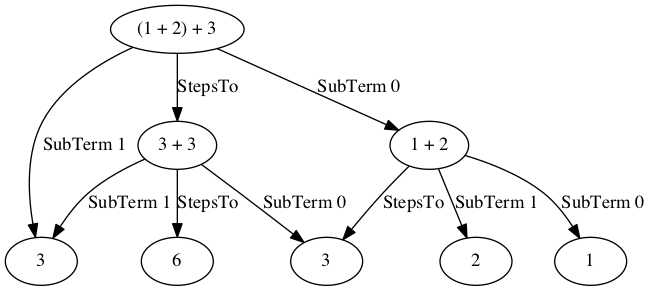
\includegraphics[width=\linewidth]{simple.png}
% \caption{The reduction graph for \texttt{1 + 2 + 3}.}
% \label{fig:simple-reduction}
% \end{figure}
% %
% We choose this graph representation instead of a simple, linear sequence
% of expressions because it will allow us to express a variety of
% traversals, such as ``step into'' and ``step over'' -- commonly found in
% traditional debuggers.

\subsection{Reduction Graphs}

\subsection{Tracing Semantics}
\label{sec:inter-semant}
%
\begin{figure*}[t]
\relDescription{Trace Syntax}
$$
\begin{array}{rrcl}
  & \tr & ::= & \bullet \spmid \singlestep{e}{e}; \tr \spmid \subterm{e}{e}; \tr
\end{array}
$$
\\
\relDescription{\subtermssym}
\begin{gather*}
\begin{array}{lcl}
\subtermssym                 & \dcolon & e \to \tr \\
\subterms{\eapp{e_1}{e_2}}   & \defeq & \subterm{\eapp{e_1}{e_2}}{e_1}; \subterm{\eapp{e_1}{e_2}}{e_2} \\
\subterms{\eplus{e_1}{e_2}}   & \defeq & \subterm{\eplus{e_1}{e_2}}{e_1}; \subterm{\eplus{e_1}{e_2}}{e_2} \\
\subterms{\eif{e_1}{e_2}{e_3}}   & \defeq & \subterm{\eif{e_1}{e_2}{e_3}}{e_1}; \\
                                &        & \subterm{\eif{e_1}{e_2}{e_3}}{e_2}; \\
                                &        & \subterm{\eif{e_1}{e_2}{e_3}}{e_3} \\
\subterms{\elet{x}{e_1}{e_2}}   & \defeq & \subterm{\elet{x}{e_1}{e_2}}{e_1}; \\
                                &        & \subterm{\elet{x}{e_1}{e_2}}{e_2} \\
\subterms{\efun{x}{e}}       & \defeq & \subterm{\efun{x}{e}}{e} \\
\subterms{e}                 & \defeq & \bullet
\end{array}
\end{gather*}
\judgementHead{Evaluation}{\stepg{e}{\su}{\tr}{e}{\su}{\tr}}
\begin{gather*}
\inference[\recontext]
  {\stepg{e}{\su}{\tr}{e_1}{\su_1}{\tr_1}}
  {\stepg{C[e]}{\su}{\tr}{C[e_1]}{\su_1}{\singlestep{C[e]}{C[e_1]}; \subterms{C[e_1]}; \tr_1}}
\\ \\
\inference[\reappgood]
  {\pair{\efun{x}{e}}{\su_2} = \force{v_1}{\tfun{\thole{}}{\thole{}}}{\su_1}}
  {\stepg{\eapp{v_1}{v_2}}{\su_1}{\tr}
         {e\sub{x}{v_2}}{\su_1;\su_2}{\singlestep{\eapp{v_1}{v_2}}{e\sub{x}{v_2}}; \subterms{e\sub{x}{v_2}}; \tr}}
\\ \\
\inference[\reappbad]
  {\pair{\stuck}{\su_2} = \force{v_1}{\tfun{\thole{}}{\thole{}}}{\su_1}}
  {\stepg{\eapp{v_1}{v_2}}{\su_1}{\tr}{\stuck}{\su_1;\su_2}{\singlestep{\eapp{v_1}{v_2}}{\stuck}; \tr}}
\end{gather*}
\caption{A selection of the operational semantics from
  Figure~\ref{fig:operational}, extended to collect a full reduction
  graph.}
\label{fig:interactive}
\end{figure*}
%
The changes to the operational semantics of \S~\ref{sec:semantics} are
mechanical, so we will not reproduce them in full; instead we describe
the procedure for extending a transition rule and provide a selection of
examples in Figure~\ref{fig:interactive}.

First, we extend the transition relation to collect a set of edges from
which we will construct the graph.
%
An edge between two expressions is either a ``steps-to'' edge -- written
\singlestep{e_1}{e_2} -- indicating that $e_1$ transitions to $e_2$ in a
single step, or a ``sub-term'' edge -- written \subterm{e_1}{e_2} --
indicating that $e_1$ contains $e_2$ as a sub-expression.
%
Collecting the steps-to edges is a simple matter of recording the
consequent of each original rule in the trace; each original judgment
\step{e_1}{\su_1}{e_2}{\su_2} becomes
\stepg{e_1}{\su_1}{\tr_1}{e_2}{\su_2}{\singlestep{e_1}{e_2}; \tr_1}.
%
The sub-term edges can be delegated to a new \subtermssym helper
function, which adds edges from an expression to each of its
\emph{immediate} sub-expressions.
%
We collect new sub-term edges after each transition, thus the final
template for the small-step relation is:
\[
\stepg{e_1}{\su_1}{\tr_1}{e_2}{\su_2}{\singlestep{e_1}{e_2}; \subterms{e_2}; \tr_1}
\]

After evaluation the reduction graph can be constructed directly from
the trace $\tr$ as follows:
\[
G(\tr) = \pair{\{e \spmid e \in \tr\}}{\tr}
\]

% \subsection{Traversing the Reduction Graph}
\subsection{Interactive Debugging}
\label{sec:traversing-graph}

Given a reduction graph $G$ and an initial path
$p = \singlestep{e_1}{\singlestep{e_2}{e_n}}$, such that
\stepsg{e_1}{\emptysu}{\bullet}{e_n}{\su}{\tr}, we define the following
traversals in Figure~\ref{fig:traversing-graph}:
%
\begin{itemize}
\item \stepforwardsym takes a single step forward.
\item \stepbackwardsym takes a single step backward.
\item \jumpforwardsym takes a ``big'' step forward to the next function call.
\item \jumpbackwardsym takes a ``big'' step backward to the previous function call.
\item \stepintosym steps into a function call in a sub-term, isolating it from the context.
\item \stepoversym steps over a function call in a sub-term.
\end{itemize}
%
The initial path $p$ is required for the backward-steps as a node may
have multiple incoming $\leadsto$ edges, \eg
\singlestep{\eplus{1}{2}}{3} and \singlestep{\eplus{2}{1}}{3}.
%
The sub-term edges $\searrow$ allow us to decompose an expression into a
sub-expression and the surrounding context, thus enabling the \stepintosym
and \stepoversym traversals.
%


\begin{figure*}[t]
\centering
\[
\begin{array}{lcl}
\stepforward{G}{p}{e_i}  &\defeq& \left\{\begin{array}{ll}
    e_j, & \text{where } \singlestep{e_i}{e_j} \in G
                         \end{array}\right\} \\ \\
\stepbackward{G}{p}{e_i}  &\defeq& \left\{\begin{array}{ll}
    e_j, & \text{where } \singlestep{e_j}{e_i} \in G \text{ and } e_j \in p
                         \end{array}\right\} \\ \\
\jumpforward{G}{p}{e_i} &\defeq& \text{let } e_j = \stepforward{G}{p}{e_i} \text{ in }
                         \left\{\begin{array}{ll}
                         e_j, & \text{if } e_j = \eapp{v_1}{v_2} \\
                         \jumpforward{G}{p}{e_{j}}, & \text{otherwise}
                         \end{array}\right\} \\ \\
\jumpbackward{G}{p}{e_i} &\defeq& \text{let } e_j = \stepbackward{G}{p}{e_i} \text{ in }
                         \left\{\begin{array}{ll}
                         e_j, & \text{if } e_j = \eapp{v_1}{v_2} \\
                         \jumpbackward{G}{p}{e_{j}}, & \text{otherwise}
                         \end{array}\right\} \\ \\
\stepinto{G}{p}{e_i} &\defeq& \left\{\begin{array}{ll}
                         e\sub{x}{v_2}, & \text{if } e_i = C[\eapp{v_1}{v_2}] \text{ and } \singlestep{\eapp{v_1}{v_2}}{e\sub{x}{v_2}}
                         \end{array}\right\} \\ \\
\stepover{G}{p}{e_i} &\defeq& \left\{\begin{array}{ll}
                         C[v], & \text{if } e_i = C[\eapp{v_1}{v_2}] \text{ and } \multistep{\eapp{v_1}{v_2}}{v}
                         \end{array}\right\}
\end{array}
\]
\caption{Rules for traversing the reduction graph given a path and
  node. \stepintosym and \stepoversym require a traversal of the
  sub-term edges to decompose $e_i$ into the target expression
  \eapp{v_1}{v_2} and the context $C$.  \ES{these rules are quite ugly and waste space..} }
\label{fig:traversing-graph}
\end{figure*}


% \begin{itemize}
% \item extend operational semantics to collect reduction graph
% \item nodes are terms, edges indicate ``steps-to'' and ``sub-term'' relations
% \item visualize path through reduction graph
% \item expand edges to reveal more fine-grained steps (step/jump forward/backward)
% \item never lose context (unlike traditional debugger)
% \end{itemize}
